\documentclass[compress]{beamer}        % [compress] (written before {beamer} <=> navigation bar one line, all subsections in 1 line instead of 2

% Setup appearance:
\usetheme{CambridgeUS}
%	AnnArbor | Antibes | Bergen |
%	Berkeley | Berlin | Boadilla |
%	boxes | CambridgeUS | Copenhagen |
%	Darmstadt | default | Dresden |
%	Frankfurt | Goettingen |Hannover |
%	Ilmenau | JuanLesPins | Luebeck |
%	Madrid | Malmoe | Marburg |
%	Montpellier | PaloAlto | Pittsburgh |
%	Rochester | Singapore | Szeged |
%	Warsaw
%

\useoutertheme[footline=authorinstitute,subsection=false]{miniframes}
\usecolortheme{whale}

%	albatross | beaver | beetle |
%	crane | default | dolphin |
%	dove | fly | lily | orchid |
%	rose |seagull | seahorse |
%	sidebartab | structure |
%	whale | wolverine


\setbeamertemplate{footline}
{
  \hbox{%
  \begin{beamercolorbox}[wd=.25\paperwidth,ht=2.25ex,dp=1ex,center]{title in head/foot}%
    \usebeamerfont{date in head/foot}\insertshortauthor
  \end{beamercolorbox}%
  \begin{beamercolorbox}[wd=.5\paperwidth,ht=2.25ex,dp=1ex,center]{date in head/foot}%
    \usebeamerfont{title in head/foot}\insertshortinstitute
  \end{beamercolorbox}%
  \begin{beamercolorbox}[wd=.25\paperwidth,ht=2.25ex,dp=1ex,center]{title in head/foot}%
    \usebeamerfont{date in head/foot}
    \insertframenumber{} / \inserttotalframenumber
    %\insertframenumber{} / \insertpresentationendpage
  \end{beamercolorbox}}%
  \vskip0pt%
}

%\setbeamercolor{titlelike}{parent=structure}
%\setbeamercolor{structure}{fg=beamer@blendedblue}
%% \useinnertheme{rounded}
%\setbeamerfont{block title}{size={}}
%\usefonttheme[onlylarge]{structurebold}   % title and words in the table of contents bold
%\setbeamerfont*{frametitle}{size=\normalsize,series=\bfseries}
\setbeamertemplate{navigation symbols}{}
\setbeamercolor{frametitle}{parent=boxes, bg=white}
{ % only on titlepage


\usepackage{times}
\usepackage{amsmath,amssymb,amsthm}
\usepackage{color}
\usepackage{changepage}
\usepackage{multirow}
\usepackage[absolute,overlay]{textpos}
\usepackage{enumerate}
%\usepackage{pgfpages}
\usepackage[all]{xy}
\usepackage{textcomp}
\usepackage{etex}
\usepackage{tikz}
\usetikzlibrary{shapes}
%\usepackage{handoutWithNotes}
%\pgfpagesuselayout{4 on 1}[border shrink=1mm]




\definecolor{camblue}{RGB}{26,26,89}
\definecolor{Rblue}{RGB}{0,255,255}
\definecolor{Rdarkblue}{RGB}{0,0,255}
\definecolor{Rgreen}{RGB}{0,205,0}
\definecolor{green2}{RGB}{51,204,51}
\newcommand{\tcb}{\textcolor{beamer@blendedblue}}
\newcommand{\tcbb}{\textcolor{camblue}}
\newcommand{\tcr}{\textcolor{red}}
\newcommand{\tcg}{\textcolor{gray}}
\newcommand{\tcgr}{\textcolor{green2}}
\newcommand{\tcblk}{\textcolor{black}}
\newcommand{\tcRg}{\textcolor{Rgreen}}
\newcommand{\tcRdb}{\textcolor{Rdarkblue}}
\newcommand{\tcRb}{\textcolor{Rblue}}
\newcommand{\tcw}{\textcolor{white}}
\newcommand{\m}{\phantom{-}}
\newcommand{\bp}{\tcbb{$\bullet$}\:}


\title{{\huge Statistics for Computing\\[0.1cm]MA4413}}
\author[Kevin Burke]{{\bf\\[0.5cm]{\huge Lecture 3}\\[0.2cm]\emph{Probability: Definitions, Set Notation, Complement Rule, Addition Rule and Multiplication Rule}\\[1.4cm]Kevin Burke}\\[0.3cm]\tcb{kevin.burke@ul.ie}}

\institute[University of Limerick, Maths \& Stats Dept]{}
\date{}

%\TPGrid[5mm,5mm]{1}{1}

\begin{document}


\begin{frame}[t]
\titlepage
\end{frame}


\section{Definitions}
\subsection{Definitions}
\begin{frame}{\bf \tcb{Definitions}}
\begin{itemize}\itemsep1cm
\item {\bf Experiment}: any process which generates various outcomes.
\item {\bf Outcome}: one possible result of the experiment.
\item {\bf Sample Space}: the set of \emph{all} possible outcomes, denoted by $S$.
\item {\bf Event}: any subset of the sample space.
\end{itemize}

\end{frame}

\subsection{Example: Flipping Two Coins}
\begin{frame}{\bf \tcb{Example: Flipping Two Coins}}
\begin{itemize}\itemsep0.6cm
\item Experiment: flipping two coins.
\item Outcome: the results showing on the coins.
\item Sample Space: $S = \{HH, TH, HT, TT\}$.
\item Event (examples):
\begin{itemize}\itemsep0.1cm
\item ``At least one head showing'' $= \{HH, TH, HT\}$.
\item ``Getting two tails'' $= \{TT\}$.
\item ``The same result on both coins'' $= \{HH, TT\}$.
\item ``The coins show different results'' $= \{TH, HT\}$.
\end{itemize}
\end{itemize}
\end{frame}

\subsection{Probability}
\begin{frame}{\bf \tcb{Probability}}
\begin{itemize}\itemsep0.6cm
\item {\bf Probability}: the proportion (i.e., relative frequency) of times that a particular event occurs in the \emph{long run} (after repeating the experiment many times).\\[0.5cm]
\end{itemize}
Let $A$ be the symbol for the event in question. The probability of $A$ is\\[-0.2cm]
\begin{align*}
\boxed{\Pr(A) = \frac{\#(A)}{\#(S)}}\\[-0.4cm]
\end{align*}
where $\#(A)$ is the number of outcomes contained in $A$ and $\#(S)$ is the number of \emph{all possible outcomes}, i.e., the number of outcomes in the sample space.

\end{frame}



\subsection{Probability}
\begin{frame}{\bf \tcb{Probability}}

Probability \emph{must be} {\bf between zero and one}:\\[0.3cm]
\begin{itemize}\itemsep0.6cm
\item $\Pr(A) = 0$: the event $A$ is impossible.
\item $\Pr(A) = 1$: the event $A$ is certain.\\[0.6cm]
\end{itemize}
The probability value is a measure of \emph{how likely} the event is, e.g.,\\[0.1cm]
\begin{itemize}\itemsep0.2cm
\item $\Pr(A) = 0.01$: highly unlikely.
\item $\Pr(A) = 0.3$: unlikely.
\item $\Pr(A) = 0.5$: there is a 50-50 chance.
\item $\Pr(A) = 0.7$: likely.
\item $\Pr(A) = 0.99$: highly likely.
\end{itemize}

\end{frame}


\subsection{Example: Flipping Two Coins}
\begin{frame}{\bf \tcb{Example: Flipping Two Coins}}

Here $S = \{HH, TH, HT, TT\}$ $\Rightarrow$ $\#(S) = 4$.\\[0.4cm]
Consider the following events:\\[0.1cm]
\begin{itemize}\itemsep0.6cm
\item A = ``At least one head showing'' $= \{HH, TH, HT\}$.\newline
$\#(A) = 3$ $\Rightarrow$ $\Pr(A) = \tfrac{3}{4} = 0.75$.
\item B = ``Getting two tails'' $= \{TT\}$.\newline
$\#(B) = 1$ $\Rightarrow$ $\Pr(B) = \tfrac{1}{4} = 0.25$.
\item C = ``The same result on both coins'' $= \{HH, TT\}$.\newline
$\#(C) = 2$ $\Rightarrow$ $\Pr(C) = \tfrac{2}{4} = \tfrac{1}{2} = 0.5$.
\item D = ``The coins show different results'' $= \{TH, HT\}$.\newline
$\#(D) = 2$ $\Rightarrow$ $\Pr(D) = \tfrac{2}{4} = \tfrac{1}{2} = 0.5$.
\end{itemize}

\end{frame}



\subsection{Complement Rule}
\begin{frame}{\bf \tcb{Complement Rule}}
Either the event $A$ happens or it does not happen.\\[0.8cm]
In the latter case, $A^c$ (pronounced ``A-complement'') occurs instead - $A^c$ the event which is the opposite of $A$.\\[0.8cm]
The {\bf complement rule} states that
\begin{align*}
\boxed{\Pr(A^c) = 1 - \Pr(A)}.\\[-0.2cm]
\end{align*}
For example, if $\Pr(\text{light bulb fails}) = 0.05$, then $\Pr(\text{light bulb works)} = 1 - \Pr(\text{light bulb fails}) = 1 - 0.05 = 0.95.$
\end{frame}


\subsection{Question 1}
\begin{frame}{\bf \tcb{Question 1}}

Consider the experiment where both a die is rolled and a coin is flipped.\\[0.2cm]
\begin{enumerate}[a)]\itemsep0.2cm
\item What is the sample space for this experiment?
\item Calculate $\Pr(\text{getting a head and any number})$.
\item Calculate $\Pr(\text{getting a head and a six})$.
\item Calculate $\Pr(\text{getting a head and an \emph{even} number})$.
\item Calculate $\Pr(\text{getting a tail and a number \emph{greater than} four})$.\\{\footnotesize(greater than four $\Rightarrow$ five or six)}
\item What is the probability of getting \emph{two} heads and a six?
\end{enumerate}

\end{frame}

\subsection{R Code}
\begin{frame}{\bf \tcb{R Code}}

The \texttt{expand.grid} function in R is useful for finding all outcomes in a sample space:\\[0.2cm]
\begin{tabular}{|l|}
\hline
\texttt{coin = c("H","T")}\\
\texttt{die = c(1,2,3,4,5,6)}\\[0.4cm]
\texttt{expand.grid(coin,coin) \# two coins}\\
\texttt{expand.grid(coin,coin,coin) \# three coins}\\
\texttt{expand.grid(coin,coin,coin,coin) \# four coins}\\
\texttt{expand.grid(coin,die) \# coin and a die}\\
\texttt{expand.grid(die,die) \# two dice}\\
\hline
\multicolumn{1}{c}{}\\[-0.1cm]
\end{tabular}

\end{frame}


\section{Set Notation}
\subsection{Set Notation}
\begin{frame}{\bf \tcb{Set Notation}}
If $A$ and $B$ are two events then we have\\[0.2cm]
\begin{itemize}\itemsep0.2cm
\item {\boldmath$A \cup B$}: ``A union B'' represents A or B or \emph{both together}, i.e., $A \cup B =$ at least one of the two occurs.
    \begin{center}
    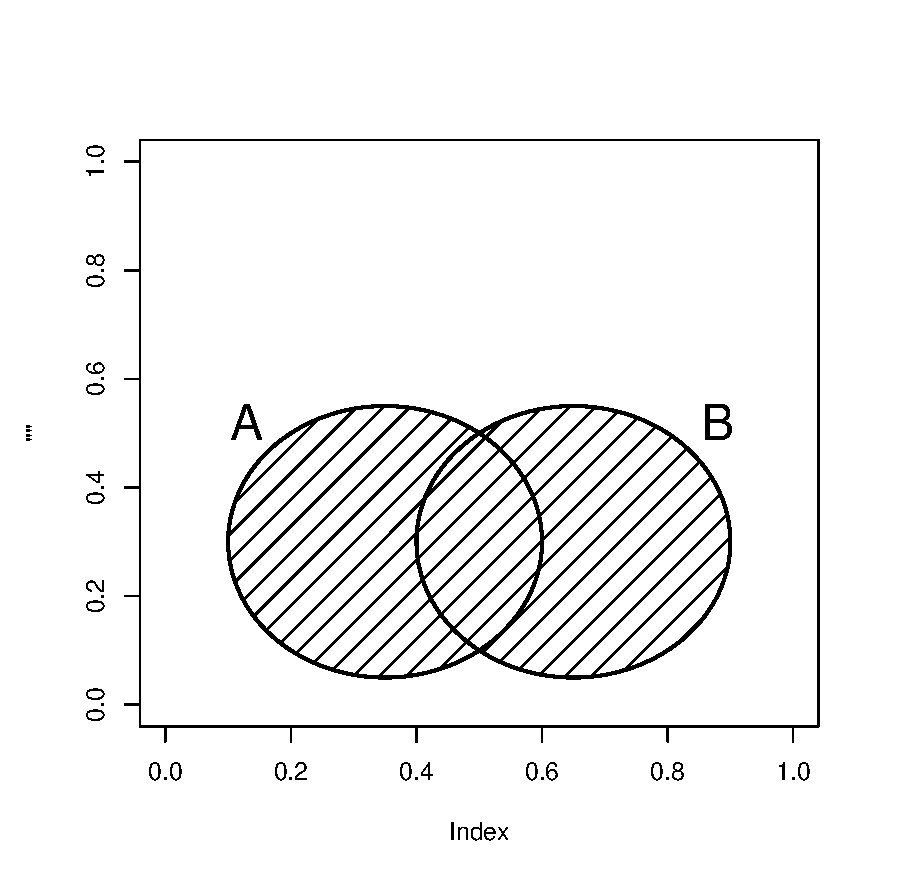
\includegraphics[width=0.3\textwidth, trim = 3.5cm 3.4cm 2.5cm 6cm, clip]{Union}
    \end{center}
\item {\boldmath$A \cap B$}: ``A intersection B'' represents A \emph{and} B, i.e., $A \cap B =$ both occur together.
    \begin{center}
    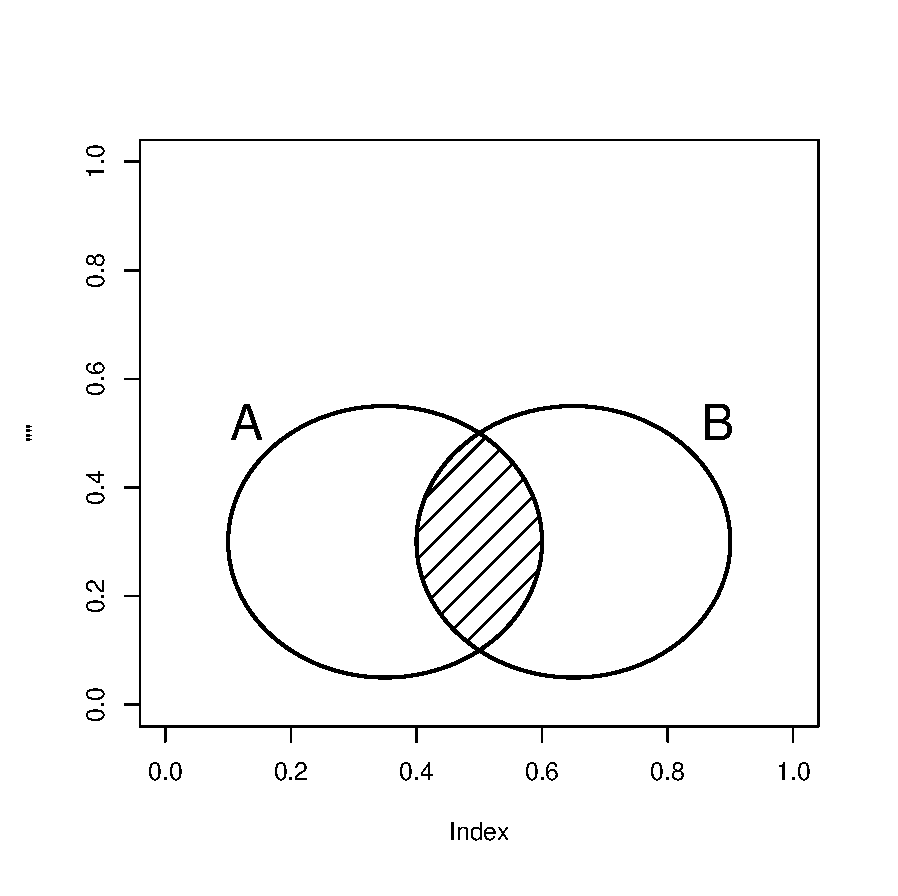
\includegraphics[width=0.3\textwidth, trim = 3.5cm 3.4cm 2.5cm 6cm, clip]{Intersect}
    \end{center}
\end{itemize}
\end{frame}



\subsection{Example: Flipping Two Coins}
\begin{frame}{\bf \tcb{Example: Flipping Two Coins}}
$A =$ ``At least one head showing'' $= \{HH, TH, HT\}$.\\[0.2cm]
$C =$ ``The same result on both coins'' $= \{HH, TT\}$.
\begin{center}
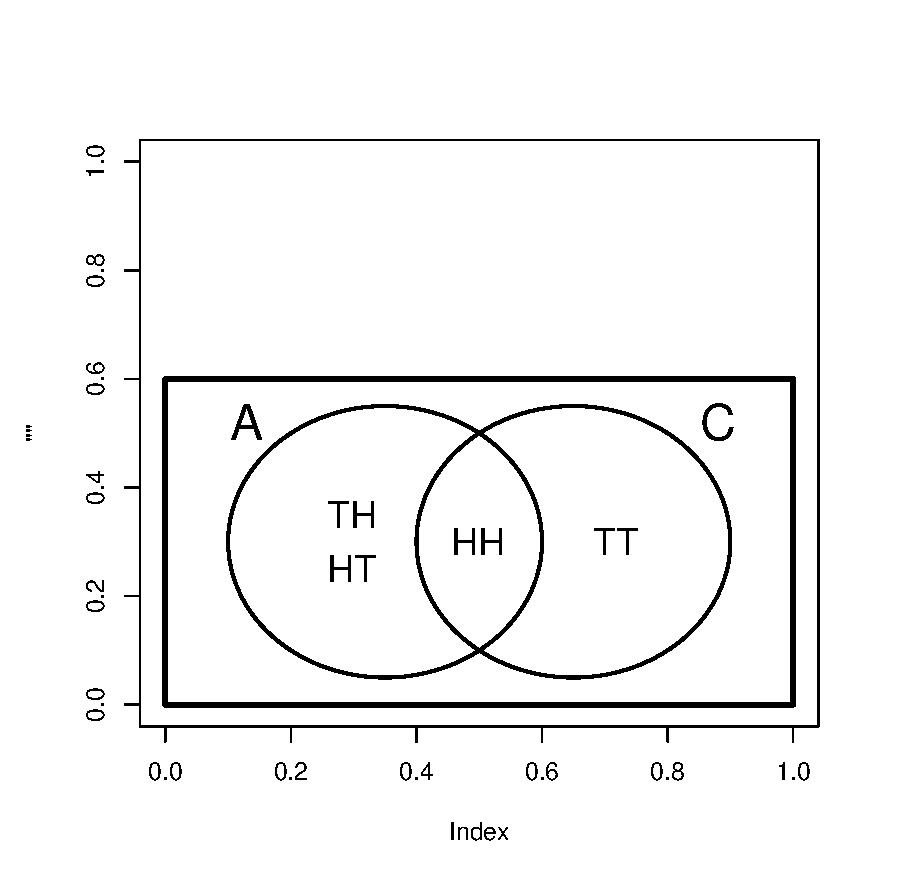
\includegraphics[width=0.4\textwidth, trim = 2.2cm 2.9cm 1.4cm 6cm, clip]{TwoCoins}
\end{center}
$A \cup C = \{HH, TH, HT, TT\}$ $\Rightarrow$ $\Pr(A \cup C) = \tfrac{4}{4} = 1$.\\[0.2cm]
$A \cap C = \{HH\}$ $\Rightarrow$ $\Pr(A \cap C) = \tfrac{1}{4}$.

\end{frame}


\subsection{Example: Flipping Two Coins}
\begin{frame}{\bf \tcb{Example: Flipping Two Coins}}\label{vennexample}
$B =$ ``Getting two tails'' $= \{TT\}$.\\[0.2cm]
$C =$ ``The same result on both coins'' $= \{HH, TT\}$.
\begin{center}
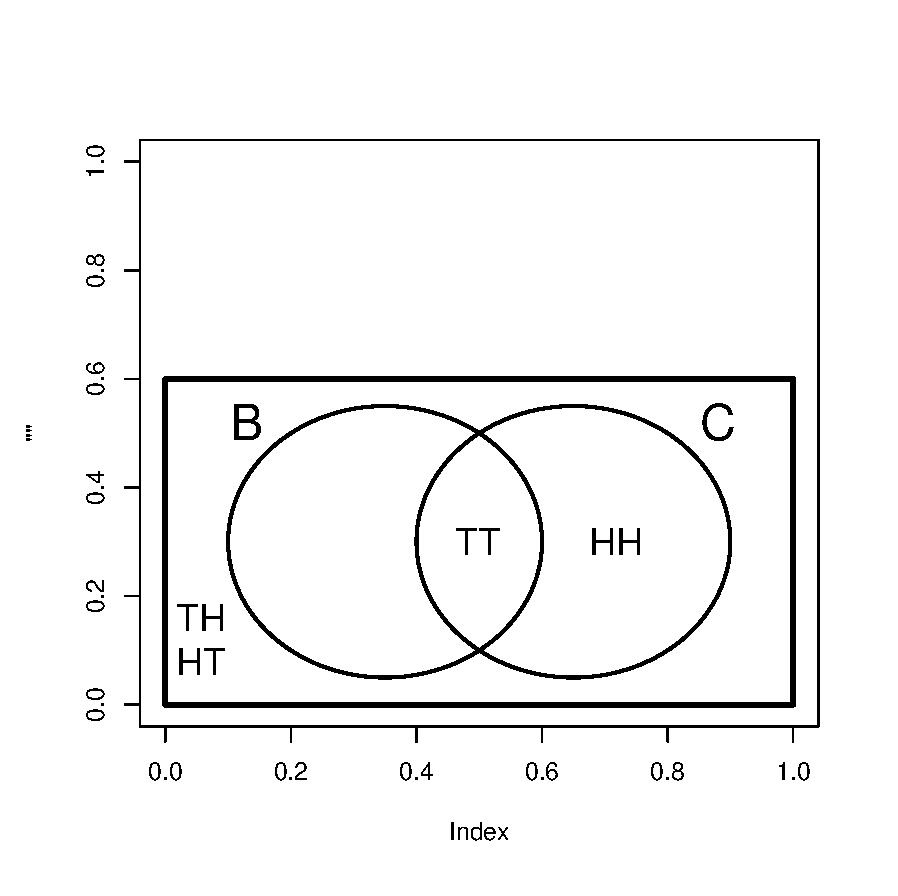
\includegraphics[width=0.4\textwidth, trim = 2.2cm 2.9cm 1.4cm 6cm, clip]{TwoCoins2}
\end{center}
$B \cup C = \{HH, TT\}$ $\Rightarrow$ $\Pr(B \cup C) = \tfrac{2}{4} = \tfrac{1}{2}$.\\[0.2cm]
$B \cap C = \{TT\}$ $\Rightarrow$ $\Pr(B \cap C) = \tfrac{1}{4}$.

\end{frame}




\section{Addition Rule}
\subsection{Addition Rule: Two Events}
\begin{frame}{\bf \tcb{Addition Rule: Two Events}}
For two events, $A$ and $B$, the probability of \emph{at least one} occurring is
\begin{align*}
\boxed{\Pr(A \cup B) = \Pr(A) + \Pr(B) - \Pr(A \cap B)}.\\
\end{align*}
Note that the intersection probability is subtracted once since it was added twice:\vspace{-0.6cm}
\begin{center}
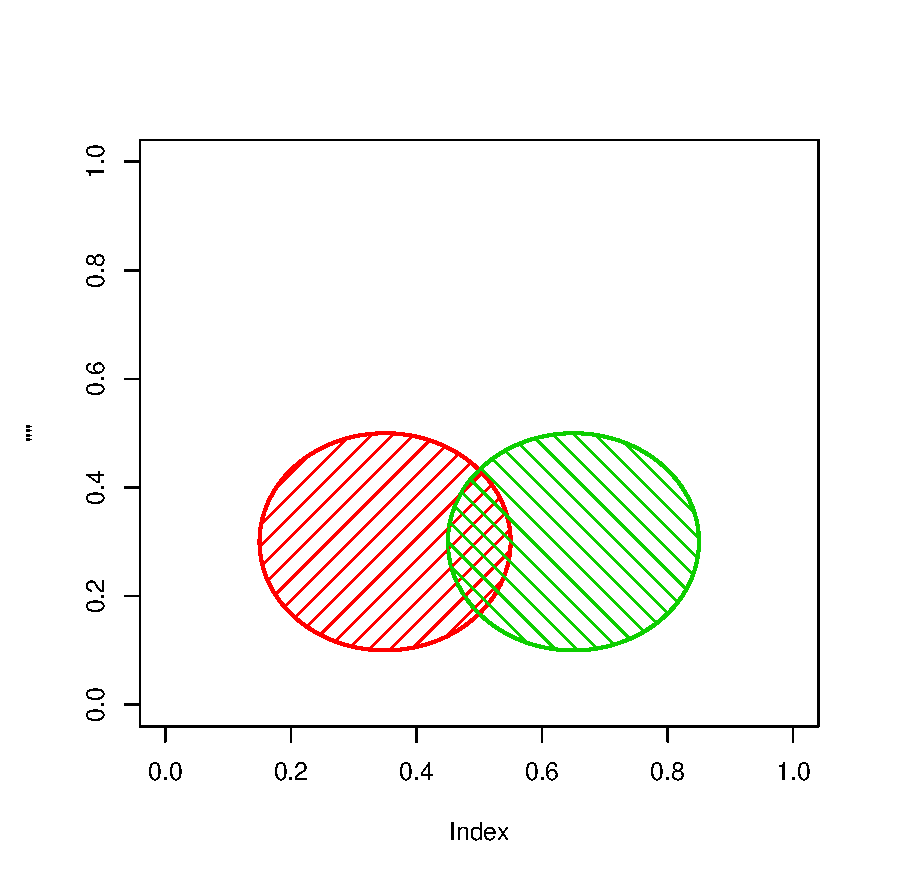
\includegraphics[width=0.5\textwidth, trim = 3.3cm 3.8cm 2.3cm 6cm, clip]{AdditionRule}
\end{center}

\end{frame}


\subsection{Addition Rule: Two Mutually Exclusive Events}
\begin{frame}{\bf \tcb{Addition Rule: Two Mutually Exclusive Events}}

$A$ and $B$ are {\bf mutually exclusive} events if they \emph{cannot} occur simultaneously, i.e., the presence of one \emph{excludes} the presence of the other $\Rightarrow$ $\boxed{\Pr(A \cap B) = 0}$.\vspace{-0.5cm}

\begin{center}
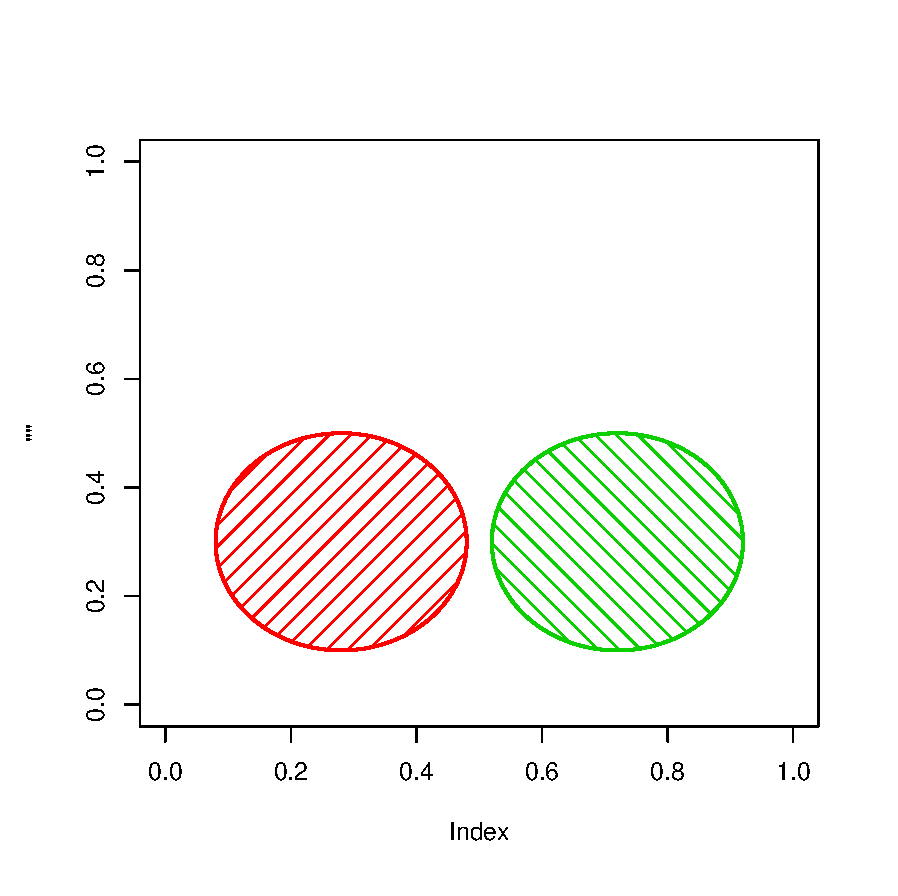
\includegraphics[width=0.5\textwidth, trim = 3.3cm 3.8cm 2.3cm 6cm, clip]{AdditionRuleMutuallyExclusive}
\end{center}

In this case the previous formula simplifies to
\begin{align*}
\Pr(A \cup B) = \Pr(A) + \Pr(B)
\end{align*}
since $\Pr(A \cap B) = 0$.

\end{frame}

\subsection{More than Two Events}
\begin{frame}{\bf \tcb{More than Two Events}}
For \emph{three} events, $A$, $B$ and $C$, the probability of \emph{at least one} occurring is
\begin{align*}
\Pr(A \cup B \cup C) &= \Pr(A) + \Pr(B) + \Pr(C)\\
 &\qquad- \Pr(A \cap B) - \Pr(A \cap C) - \Pr(B \cap C)\\
 &\qquad+ \Pr(A \cap B \cap C).\\[-0.9cm]
\end{align*}
\begin{minipage}[b]{0.5\textwidth}
Can you see why from the diagram?\\[1.1cm]
{\footnotesize(clearly the situation becomes complicated for more than three events - we will not deal with such situations)}
\end{minipage}
\begin{minipage}[b]{0.49\textwidth}
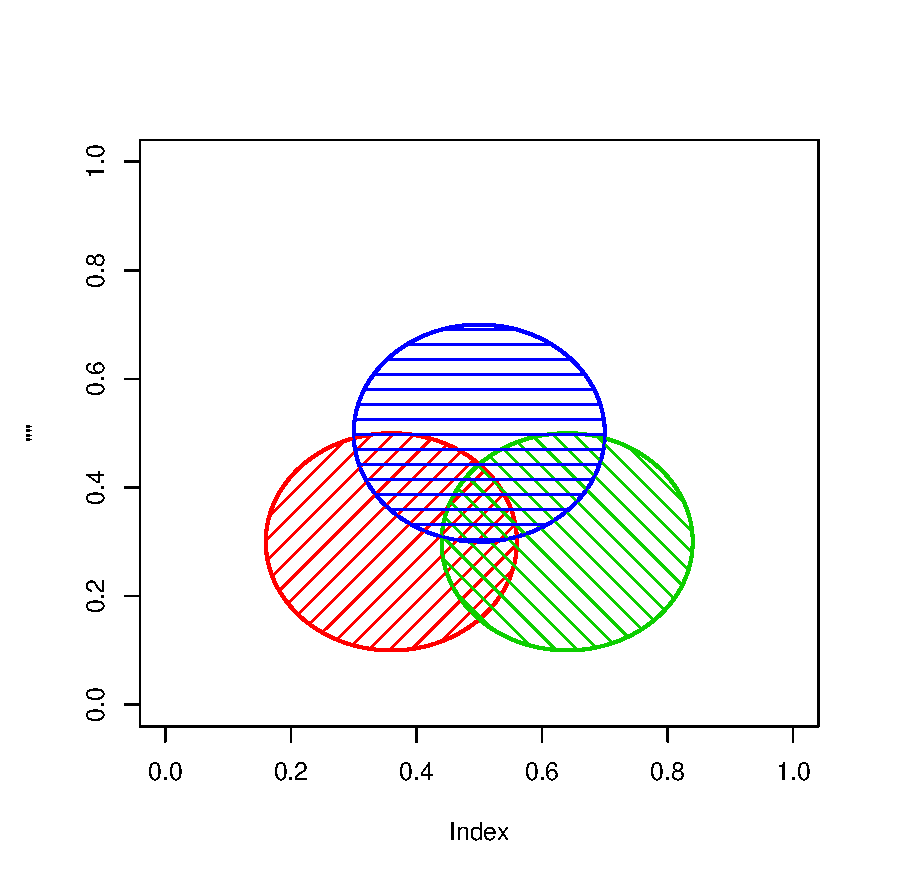
\includegraphics[width=1\textwidth, trim = 3.3cm 3.8cm 2.3cm 4.8cm, clip]{AdditionRule3}
\end{minipage}

\end{frame}


\subsection{More than Two Mutually Exclusive Events}
\begin{frame}{\bf \tcb{More than Two Mutually Exclusive Events}}
For \emph{three} mutually exclusive events, the previous formula simplifies to
\begin{align*}
\Pr(A \cup B \cup C) &= \Pr(A) + \Pr(B) + \Pr(C)\\[-0.5cm]
\end{align*}
as \emph{all} intersections have zero probability since the events cannot happen simultaneously.\\[0.5cm]

For {\boldmath$k$} {\bf mutually exclusive} events, $E_1, E_2, E_3, \ldots E_k$, it should be clear that the probability of at least one occurring is:
\begin{align*}
\boxed{\Pr(E_1 \cup E_2 \cup \cdots \cup E_k) = \Pr(E_1) + \Pr(E_2) + \cdots + \Pr(E_k)}.%\\[-0.5cm]
\end{align*}

%It should be clear from the previous slide that the above simple formula \emph{only} applies to \emph{mutually exclusive} events.

\end{frame}


\subsection{At Least One Vs None of the Events}
\begin{frame}{\bf \tcb{At Least One Vs None of the Events}}
$\Pr(A \cup B)$ is the probability of \emph{at least one} of $A$ or $B$ occurring.\\[0.5cm]

Recall from earlier that the \emph{complement rule} allows us to evaluate the probability of a complementary (i.e., opposite) event.\\[0.4cm]

The complement of ``at least one'' is ``none''. In mathematical notation: $(A \cup B)^c = A^c \cap B^c$, i.e., simultaneously not $A$ \emph{and} not $B$.\\[0.4cm]

Thus, the probability of \emph{neither $A$ nor $B$} is
\begin{align*}
\boxed{\Pr(A^c \cap B^c) = 1 - \Pr(A \cup B)}.\\[-0.2cm]
\end{align*}
Conversely, if we have $\Pr(A^c \cap B^c)$ and wish for $\Pr(A \cup B)$, we can use
\begin{align*}
\boxed{\Pr(A \cup B) = 1 - \Pr(A^c \cap B^c)}.
\end{align*}

\end{frame}


\subsection{At Least One Vs None of the Events}
\begin{frame}{\bf \tcb{At Least One Vs None of the Events}}

Of course the ideas on the previous slide hold for more than two events, i.e.,\\[-0.1cm]
\begin{align*}
\boxed{\Pr(E_1^c \cap E_2^c \cap \cdots \cap E_k^c) = 1 - \Pr(E_1 \cup E_2 \cup \cdots \cup E_k)},\\[-0.2cm]
\end{align*}
and, conversely,\\[-0.1cm]
\begin{align*}
\boxed{\Pr(E_1 \cup E_2 \cup \cdots \cup E_k) = 1 - \Pr(E_1^c \cap E_2^c \cap \cdots \cap E_k^c)}.
\end{align*}


\end{frame}


\subsection{Example: Flipping Two Coins}
\begin{frame}{\bf \tcb{Example: Flipping Two Coins}}
In the example of flipping two coins we had:\\[0.2cm]
$B =$ ``Getting two tails'' $= \{TT\}$ $\Rightarrow$ $\Pr(B) = \tfrac{1}{4} = 0.25$.\\[0.3cm]
$C =$ ``The same result on both coins'' $= \{HH, TT\}$ $\Rightarrow$ $\Pr(B) = \tfrac{2}{4} = 0.5$.\\[0.7cm]

These events are clearly \emph{not} mutually exclusive since $B \cap C = \{TT\}$ $\Rightarrow$ $\Pr(B \cap C) = \tfrac{1}{4} = 0.25$.\\[0.7cm]

To calculate the probability of ``getting two tails'' \emph{or} ``the same result'' \emph{or} both (i.e., at least one of $B$ or $C$), we can use the addition rule:\\[-0.6cm]
\begin{align*}
\Pr(B \cup C) = \Pr(B) + \Pr(C) - \Pr(B \cap C) = 0.25 + 0.5 - 0.25 = 0.5.\\[-0.4cm]
\end{align*}
{\footnotesize(note that we found this probability already using the venn diagram - see slide \pageref{vennexample})}
\end{frame}


\subsection{Example: Flipping Two Coins}
\begin{frame}{\bf \tcb{Example: Flipping Two Coins}}

If we want the probability that \emph{neither $B$ nor $C$} occurs we use the complement rule:
\begin{align*}
\Pr(B^c \cap C^c) = 1 - \Pr(B \cup C) = 1 - 0.5 = 0.5.\\[-0.2cm]
\end{align*}

{\footnotesize(Note that the above probability can be found using a more manual approach since $B^c = \{HH,TH,HT\}$ and $C^c = \{TH,HT\}$ $\Rightarrow$ $B^c \cap C^c = \{TH, HT\}$)}

\end{frame}



\subsection{Example: Rolling One Die}
\begin{frame}{\bf \tcb{Example: Rolling One Die}}
Consider the experiment of rolling a die which has $S = \{1,2,3,4,5,6\}$.\\[0.3cm]

We then define the events:
\begin{itemize}
\item $E_1 = \text{``the result is a one''} = \{1\}$ $\Rightarrow$ $\Pr(E_1) = \tfrac{1}{6}$.
\item $E_2 = \text{``the result is a two''} = \{2\}$ $\Rightarrow$ $\Pr(E_2) = \tfrac{1}{6}$.
\item $E_3 = \text{``the result is a three''} = \{3\}$ $\Rightarrow$ $\Pr(E_3) = \tfrac{1}{6}$.
\item $E_4 = \text{``the result is a four''} = \{4\}$ $\Rightarrow$ $\Pr(E_4) = \tfrac{1}{6}$.
\item $E_5 = \text{``the result is a five''} = \{5\}$ $\Rightarrow$ $\Pr(E_5) = \tfrac{1}{6}$.
\item $E_6 = \text{``the result is a six''} = \{6\}$ $\Rightarrow$ $\Pr(E_6) = \tfrac{1}{6}$.\\[0.5cm]
\end{itemize}

These events are all \emph{mutually exclusive} since, for example, the result cannot \emph{simultaneously} be a one \emph{and} a two.

\end{frame}


\subsection{Example: Rolling One Die}
\begin{frame}{\bf \tcb{Example: Rolling One Die}}

We can add the event probabilities without worrying about intersections since they are mutually exclusive events, e.g.:\\[-0.3cm]
\begin{align*}
\Pr(\text{``result between three and five''}) &= \Pr(E_3 \cup E_4 \cup E_5) \\&= \Pr(E_3) + \Pr(E_4) + \Pr(E_5) \\
&= \tfrac{1}{6} + \tfrac{1}{6} + \tfrac{1}{6} = \tfrac{3}{6} = \tfrac{1}{2}.\\[-1.1cm]
\end{align*}

\begin{align*}
\Pr(\text{``greater than four''}) = \Pr(\text{``a five or a six''}) &= \Pr(E_5 \cup E_6) \\&= \Pr(E_5) + \Pr(E_6) \\
&= \tfrac{1}{6} + \tfrac{1}{6} = \tfrac{2}{6} = \tfrac{1}{3}.\\[-0.1cm]
\end{align*}

Finally, an example of the usefulness of the complement rule:
\begin{align*}
\Pr(\text{``less than or equal to four''}) &= 1 - \Pr(\text{``greater than four''}) \\
&= 1 - \tfrac{1}{3} = \tfrac{2}{3}.
\end{align*}

\end{frame}



\subsection{Exhaustive Events}
\begin{frame}{\bf \tcb{Exhaustive Events}}

It is worth noting that in the last example\\[-0.3cm]

\begin{align*}
\Pr(E_1 \cup E_2 \cup E_3 \cup E_4 \cup E_5 \cup E_6)& \\[0.2cm]
&\hspace{-3.5cm}= \Pr(E_1) + \Pr(E_2) + \Pr(E_3) + \Pr(E_4) + \Pr(E_5) + \Pr(E_6)\\
&\hspace{-3.5cm}= \tfrac{1}{6} + \tfrac{1}{6} + \tfrac{1}{6} + \tfrac{1}{6} + \tfrac{1}{6} + \tfrac{1}{6} \\
&\hspace{-3.5cm}= 1.\\
\end{align*}
Such events are called {\bf exhaustive} as they cover the whole sample space, i.e., they \emph{exhaust all possibilities}.\\[0.5cm]

{\footnotesize(this is important later for the \emph{law of total probability})}


\end{frame}



\subsection{Question 2}
\begin{frame}{\bf \tcb{Question 2}}
Consider the experiment where both a die is rolled and a coin is flipped (considered earlier in Question 1). Let $A = $ ``head \& even number'', \\$B =$ ``head \& any number'', $C =$ ``any face \& a five''.\\[0.3cm]
\begin{enumerate}[a)]\itemsep0.2cm
\item $A =\{H2,H4,H6\}$. Write out the set of outcomes in $B$ and $C$. Hence, calculate $\Pr(A)$, $\Pr(B)$ and $\Pr(C)$.
\item Write down $A \cap B$, $A \cap C$ and $B \cap C$. Hence, calculate the probabilities $\Pr(A \cap B)$, $\Pr(A \cap C)$ and $\Pr(B \cap C)$.
\item Which events are mutually exclusive?
\item Calculate $\Pr(A \cup B)$, $\Pr(A \cup C)$ and $\Pr(B \cup C)$ using the addition rule. %and using the method of part (b) (e.g., write out the set $A \cup B$ and then its probability).
\item What is the probability that the result is neither $A$ nor $B$?
\end{enumerate}

\end{frame}


\subsection{Question 3}
\begin{frame}{\bf \tcb{Question 3}}
Consider a RAID (redundant array of inexpensive disks) system where multiple hard disks are used simultaneously.\\[0.2cm]
Let's assume that we have two hard disks. Define the events $H_1 =$ ``hard disk one works'' and $H_2 =$ ``hard disk two works'' and also assume that $\Pr(H_1) = \Pr(H_2) = 0.9$. If the hard disks work \emph{independently} (more on this later), the probability that they both work is $\Pr(H_1 \cap H_2) = 0.81$.\\[0.2cm]
\begin{enumerate}[a)]\itemsep0.2cm
\item RAID-0 is a system which increases performance but only works if \emph{both} hard disks work. What is $\Pr(\text{RAID-0 works})$?
\item Calculate $\Pr(\text{RAID-0 fails})$.
\item RAID-1 is a system which does not increase performance but still works with only one working hard disk. What is $\Pr(\text{RAID-1 works})$?
\item Calculate $\Pr(\text{RAID-1 fails})$.
\end{enumerate}

\end{frame}


\subsection{Note on Question 3}
\begin{frame}{\bf \tcb{Note on Question 3}}
It may interest you to find out more about RAID systems (if you don't already know).\\[0.6cm]

You can have a look at this video: \tcb{http://youtu.be/RYBtmVMtH1g}.\\[0.2cm]
The first four minutes provide a good discussion of how RAID-0 and RAID-1 work. The rest of the video describes how you can set up these systems in practice.\\[0.6cm]

Also see wikipedia for information on various RAID systems: \tcb{http://en.wikipedia.org/wiki/RAID}.

\end{frame}





\section{Multiplication Rule}
\subsection{Multiplication Rule: Two Events}
\begin{frame}{\bf \tcb{Multiplication Rule: Two Events}}
Although we have found $\Pr(A \cap B)$ in the previous section manually, there is also a formula to calculate it:\\[-0.3cm]
\begin{align*}
\boxed{\Pr(A \cap B) = \Pr(A) \, \Pr(B\,|\,A)}.\\[-0.3cm]
\end{align*}
What is $B\,|\,A$? This is the event of $B$ \emph{given} that $A$ has happened.\\[0.3cm]
$\Pr(B\,|\,A)$ is a \emph{conditional probability} - it is the probability that $B$ occurs under the condition that $A$ has already occurred.\\[0.6cm]
We can change the order of multiplication if we like:
\begin{align*}
\Pr(A \cap B) = \Pr(B) \, \Pr(A\,|\,B).
\end{align*}
\end{frame}


\subsection{Multiplication Rule: Independent Events}
\begin{frame}{\bf \tcb{Multiplication Rule: Independent Events}}

Events are described as {\bf independent} if the occurrence of one has \emph{no effect} on the other.\\[0.2cm]
In this case $\boxed{\Pr(B\,|\,A) = \Pr(B)}$, i.e., it does not matter if $A$ has happened or not.\\[0.4cm]
For two independent events the multiplication formula simplifies to
\begin{align*}
\Pr(A \cap B) = \Pr(A) \, \Pr(B).\\[-0.3cm]
\end{align*}
Of course this extends to {\boldmath$k$} {\bf independent events}:
\begin{align*}
\boxed{\Pr(E_1 \cap E_2 \cap \cdots \cap E_k) = \Pr(E_1) \, \Pr(E_2) \,\cdots \, \Pr(E_k)}.\\
\end{align*}

{\footnotesize(for more than two \emph{non-independent} events there is no simple multiplication formula - much like the addition rule for \emph{non-mutually exclusive} events)}

\end{frame}


\subsection{Checking Independence}
\begin{frame}{\bf \tcb{Checking Independence}}

Assuming we have calculated $\Pr(A)$, $\Pr(B)$ and $\Pr(A \cap B)$ then we can check:\\[0.6cm]
\begin{itemize}\itemsep1cm
\item If $\Pr(A) \times \Pr(B) = \Pr(A \cap B)$ $\Rightarrow$ independent events.
\item If $\Pr(A) \times \Pr(B) \ne \Pr(A \cap B)$ $\Rightarrow$ non-independent events.
\end{itemize}


\end{frame}

\subsection{Question 4}
\begin{frame}{\bf \tcb{Question 4}}

In Question 2 we calculated: $\Pr(A)$, $\Pr(B)$, $\Pr(C)$, $\Pr(A\cap B)$, $\Pr(A\cap C)$ and $\Pr(B\cap C)$.\\[0.5cm]

\begin{enumerate}[a)]
\item Check if any of the events $A$, $B$ or $C$ are independent.
\end{enumerate}

\end{frame}


\subsection{Question 5}
\begin{frame}{\bf \tcb{Question 5}\\[-0.8cm]}

In Question 3 we looked at RAID systems and defined the events $H_1 = $ ``hard disk one works'' and $H_2 = $ ``hard disk two works'' with $\Pr(H_1) = \Pr(H_2) = 0.9$. We assume that $H_1$ and $H_2$ are \emph{independent}.

\begin{enumerate}[a)]\itemsep0.2cm
\item Show that the probability of both hard disks working is $\Pr(H_1 \cap H_2) = 0.81$.
\item Calculate $\Pr(\text{RAID-1 works}) = \Pr(H_1 \cup H_2)$.
\item What is the probability that hard disk one \emph{fails} (i.e., $\Pr(H_1^c)$)? What is the value of $\Pr(H_2^c)$?
\item $\Pr(H_1^c \cap H_2^c)$ is the probability that \emph{both} fail simultaneously, i.e.,  $\Pr(\text{RAID-1 fails})$. Calculate this probability using the answer to part (c) and the fact these events are independent.
\item Cheap hard disks exist with $\Pr(\text{cheap hard disk works}) = 0.6$. How many of these are needed to match the performance of the two-hard disk system described above?
\end{enumerate}

\end{frame}




\section{Independence Vs Mutual Exclusion}
\subsection{Independence Vs Mutual Exclusion}
\begin{frame}{\bf \tcb{Independence Vs Mutual Exclusion}}

{\bf Do not mix up the ideas of independence and mutual exclusion.\\[0.3cm]}
\begin{itemize}\itemsep0.3cm
\item {\bf Independent events}
\begin{itemize}\itemsep0.2cm
\item Have \emph{no effect} on each other.
\item \emph{Can} happen at the same time (but work \emph{independently} of each other).
\item Allow us to simplify the {\bf multiplication rule}.
\end{itemize}
\item {\bf Mutually exclusive events}
\begin{itemize}\itemsep0.2cm
\item \emph{Cannot} happen at the same time.
\item Certainly \emph{affect} each other since the presence of one excludes the presence of the other.
\item Allow us to simplify the {\bf addition rule}.
\end{itemize}
\end{itemize}

Bottom line: If events are independent they are not mutually exclusive. If events are mutually exclusive they are not independent.

\end{frame}

\subsection{Question 6}
\begin{frame}{\bf \tcb{Question 6}}
Classify the following pairs of events as being mutually exclusive, independent or dependent (but not mutually exclusive).\\[0.4cm]

\begin{tabular}{ccc}
         & Event $A$ & Event $B$ \\[0.2cm]
\tcb{a)} &  A coin shows a head   & The same coin shows a tail \\[0.2cm]
\tcb{b)} &  You work hard   & You get promoted \\[0.2cm]
\tcb{c)} &  You are Irish  & It rains in Japan \\[0.2cm]
\tcb{d)} &  Anti-virus out of date  & Laptop is virus-free \\[0.2cm]
\tcb{e)} &  You are in this lecture   & You are in the Stables \\[0.2cm]
\tcb{f)} &  You are in this lecture   & You are on Facebook \\[0.2cm]
\tcb{g)} &  An individual is not wealthy   & He/she drives an expensive car  \\[0.2cm]
\tcb{h)} &  One coin shows a head   & Another coin shows a head
\end{tabular}


\end{frame}





\end{document} 